% summary tex template
% (C) Copyright 2014 Sebastian Müller

\documentclass[11pt, oneside]{article}   	% use "amsart" instead of "article" for AMSLaTeX format
\usepackage{geometry}                		% See geometry.pdf to learn the layout options. There are lots.
\geometry{a4paper}                   		% ... or a4paper or a5paper or ... 
%\geometry{landscape}                		% Activate for for rotated page geometry
%\usepackage[parfill]{parskip}    		% Activate to begin paragraphs with an empty line rather than an indent
\usepackage{graphicx}				% Use pdf, png, jpg, or eps§ with pdflatex; use eps in DVI mode
								% TeX will automatically convert eps --> pdf in pdflatex		
\usepackage{amssymb}
\usepackage{amsmath}
%\usepackage[ngerman]{babel}
\usepackage[utf8]{inputenc}
\usepackage{hyperref}

\title{Summary}
\author{Author}
\date{WS 14/15}							% Activate to display a given date or no date

\begin{document}
\twocolumn
\maketitle
\tableofcontents
\noindent\rule{0.5\textwidth}{0.5pt}

\section{Introduction}
\begin{itemize}
	\item Item 1
	\item Item 2
\end{itemize}
Lorem Ipsum.

\section{Figure}
\begin{figure}[h!]
	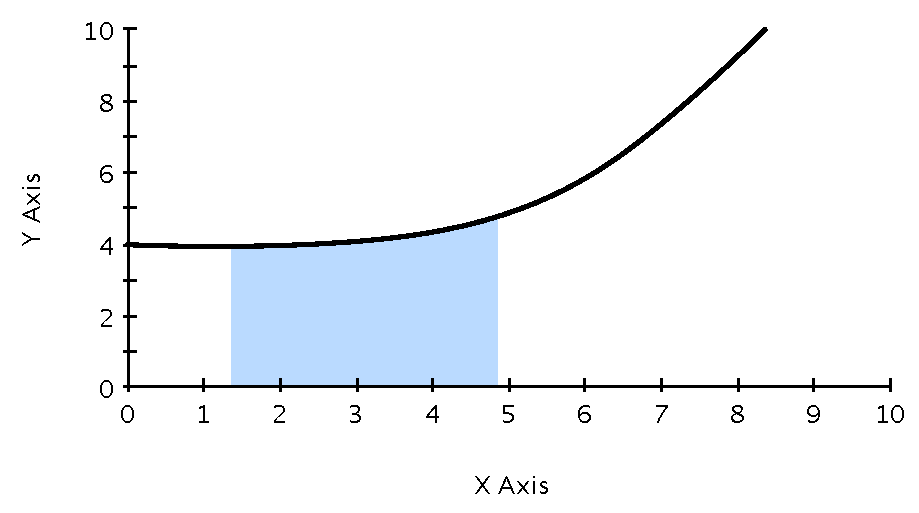
\includegraphics[width=0.5\textwidth]{figures/graph}
	\caption{A graph}
\end{figure}

\section{Equation}
\begin{align}
	\sum_{n=0}^{N-1} A_n = q
\end{align}

\end{document}  